\documentclass[12pt, oneside, a4paper]{ctexart}

\usepackage{amsmath}
\usepackage{amssymb}
\usepackage{caption}
\usepackage{float}
\usepackage[{top=2.54cm, bottom=2.54cm, left=3.18cm, right=3.18cm}]{geometry}
\usepackage{graphicx}
\usepackage[breaklinks, colorlinks=false, hidelinks]{hyperref}
\usepackage{mathptmx}
\usepackage{xcolor}
\usepackage{xeCJK}
\usepackage{tikz}

\pagestyle{empty}
\setmainfont{Times New Roman}
\setCJKmainfont[AutoFakeBold={2}]{SimSun}
\setCJKfamilyfont{zh}{SimSun}
\newCJKfontfamily\diarySong{SimSun}
\newCJKfontfamily\diaryHei{SimHei}
\newCJKfontfamily\diaryFang{FangSong}
\newCJKfontfamily\diaryShu{FZShuTi}

\newcommand{\pagecanvas}[1]{%
  \thispagestyle{empty}%
  \begin{tikzpicture}[remember picture, overlay]
    #1
  \end{tikzpicture}%
  \null
}
\newcommand{\basewest}[3]{%
  \node[anchor=base west, inner sep=0pt] at
    ([xshift=#1, yshift=-#2]current page.north west) {#3};%
}
\newcommand{\basecenter}[3]{%
  \node[anchor=base, inner sep=0pt] at
    ([xshift=#1, yshift=-#2]current page.north west) {#3};%
}
\newcommand{\northwest}[3]{%
  \node[anchor=north west, inner sep=0pt] at
    ([xshift=#1, yshift=-#2]current page.north west) {#3};%
}
\newcommand{\northcenter}[3]{%
  \node[anchor=north, inner sep=0pt] at
    ([xshift=#1, yshift=-#2]current page.north west) {#3};%
}
\newcommand{\ruleline}[3]{%
  \draw[line width=0.45pt]
    ([xshift=#1, yshift=-#3]current page.north west) --
    ([xshift=#2, yshift=-#3]current page.north west);%
}
\newcommand{\diaryFormFont}{\diaryFang\fontsize{18pt}{20pt}\selectfont}
\newcommand{\diaryBodyFont}{\diarySong\fontsize{14pt}{19pt}\selectfont}
\newcommand{\diaryJournalBodyFont}{\diarySong\fontsize{12pt}{15pt}\selectfont}
\newcommand{\diaryTableFont}{\diaryFang\fontsize{15pt}{17pt}\selectfont}
\newcommand{\diaryPageFont}{\diarySong\fontsize{16pt}{18pt}\selectfont}
\ctexset{
  section = {format = {\centering\diaryHei\bfseries\Large}},
  subsection = {format = {\diaryHei\bfseries\large}},
  subsubsection = {format = {\diaryHei\bfseries\normalsize}}
}
\newcommand{\fixedline}[1]{\noindent\makebox[0pt][l]{#1}\\}
\newcommand{\diaryDateRuleSegments}{%
  \draw[line width=0.45pt, line cap=butt]
    ([xshift=37.0mm, yshift=-54.35mm]current page.north west) --
    ([xshift=50.0mm, yshift=-54.35mm]current page.north west)
    ([xshift=55.8mm, yshift=-54.35mm]current page.north west) --
    ([xshift=65.1mm, yshift=-54.35mm]current page.north west)
    ([xshift=69.8mm, yshift=-54.35mm]current page.north west) --
    ([xshift=80.7mm, yshift=-54.35mm]current page.north west)
    ([xshift=95.0mm, yshift=-54.35mm]current page.north west) --
    ([xshift=108.0mm, yshift=-54.35mm]current page.north west)
    ([xshift=112.6mm, yshift=-54.35mm]current page.north west) --
    ([xshift=121.8mm, yshift=-54.35mm]current page.north west)
    ([xshift=126.6mm, yshift=-54.35mm]current page.north west) --
    ([xshift=137.5mm, yshift=-54.35mm]current page.north west);%
}
\newcounter{journalpagecounter}
\setcounter{journalpagecounter}{0}
\newcommand{\journalpage}{%
  \stepcounter{journalpagecounter}%
  \pagecanvas{%
    \basewest{147mm}{20mm}{\diaryPageFont 实\hspace{0.25em}习\hspace{0.25em}日\hspace{0.25em}记}
    \ruleline{31.5mm}{179mm}{26.5mm}
    \ruleline{32mm}{177mm}{273mm}
    \basewest{158mm}{280mm}{\diaryPageFont 第\hspace{0.4em}\thejournalpagecounter\hspace{0.4em}页}
  }%
}

\begin{document}

\pagecanvas{%
  \northwest{60mm}{45mm}{
\includegraphics[width=90mm]{assets/tongji-diary-logo.png}}
  \basecenter{105mm}{99mm}{\diaryShu\fontsize{56pt}{45pt}\selectfont 实习日记本}
  \basewest{42mm}{143mm}{\diaryFormFont 学\hspace{2.1em}院}
  \ruleline{78mm}{176mm}{147mm}
  \basecenter{127mm}{143mm}{\diaryFormFont 交通学院}
  \basewest{42mm}{158mm}{\diaryFormFont 专\hspace{2.1em}业}
  \ruleline{78mm}{176mm}{162mm}
  \basecenter{127mm}{158mm}{\diaryFormFont 车辆工程}
  \basewest{42mm}{173mm}{\diaryFormFont 学\hspace{2.1em}号}
  \ruleline{78mm}{176mm}{177mm}
  \basecenter{127mm}{173mm}{\diaryFormFont 2352670}
  \basewest{42mm}{188mm}{\diaryFormFont 学生姓名}
  \ruleline{78mm}{176mm}{192mm}
  \basecenter{127mm}{188mm}{\diaryFormFont 肖哲夫}
  \basewest{42mm}{203mm}{\diaryFormFont 接受单位}
  \ruleline{78mm}{176mm}{207mm}
  \basecenter{127mm}{203mm}{\diaryFormFont 中车南京浦镇车辆有限公司}
  \basewest{42mm}{218mm}{\diaryFormFont 地\hspace{2.1em}址}
  \ruleline{78mm}{176mm}{222mm}
  \basecenter{127mm}{218mm}{\diaryFormFont 南京市江北新区浦珠北路68号}
  \basewest{35mm}{233mm}{\diaryFormFont 指导教师姓名}
  \ruleline{78mm}{176mm}{237mm}
  \basecenter{127mm}{233mm}{\diaryFormFont 周凯}
}

\newpage
\pagecanvas{%
  \basecenter{105mm}{42mm}{\diaryHei\fontsize{22pt}{22pt}\selectfont 大学生校外实习守则}
  \northcenter{105mm}{62mm}{%
    \begin{minipage}{155mm}
      \diaryBodyFont
      \setlength{\parindent}{2em}
      \setlength{\parskip}{0pt}
      \par{}
      一、高校校外实习是高等教育同社会主义建设相结合的重要环节，是培养合格人才的重要保证，每个学生必须按照教学计划的要求，认真参加各种形式的校外实习活动，并自觉遵守本守则。\par{}
      二、严格遵守实习单位的有关规章制度。如有违反，学校应会同实习单位按有关规定严肃处理。\par{}
      三、自觉遵守劳动纪律、尊重实习带教人员，服从安排，严格执行安全操作规程。\par{}
      四、妥善保管实习需要而借阅的图纸、资料，严格遵守保密制度，防止泄密。\par{}
      五、认真写好实习日记，客观记录实习的内容、问题及心得。\par{}
      六、独立完成实习报告，系统总结、综合分析实习中的问题以及解决问题的方法和建议。\par{}
      七、实习结束时，必须如数归还所借用的劳防用品、工具、仪器、资料及生活用品，如有损坏或遗失应按规定赔偿。\par{}
      八、学生在实习期间造成伤残和死亡的，可按“大学生团体平安保险”有关规定给予赔偿。
    \end{minipage}
  }
}

\newpage
\pagecanvas{%
  \draw[line width=0.45pt]
  ([xshift=29mm, yshift=-31mm]current page.north west)
  rectangle
  ([xshift=180mm, yshift=-249mm]current page.north west);
  \ruleline{29mm}{180mm}{44mm}
  \ruleline{29mm}{180mm}{57mm}
  \ruleline{29mm}{180mm}{70mm}
  \ruleline{29mm}{180mm}{197mm}
  \basecenter{105mm}{40mm}{\diaryTableFont 实习起迄日期}
  \basewest{32mm}{53mm}{\diaryTableFont 自}
  \basewest{50.2mm}{53mm}{\diaryTableFont 年}
  \basewest{65.1mm}{53mm}{\diaryTableFont 月}
  \basewest{80mm}{53mm}{\diaryTableFont 日起至}
  \basewest{107mm}{53mm}{\diaryTableFont 年}
  \basewest{121.9mm}{53mm}{\diaryTableFont 月}
  \basewest{136.8mm}{53mm}{\diaryTableFont 日止}
  \basecenter{43.5mm}{53mm}{\diaryTableFont 2026}
  \basecenter{60.45mm}{53mm}{\diaryTableFont 7}
  \basecenter{75.25mm}{53mm}{\diaryTableFont 6}
  \basecenter{101.45mm}{53mm}{\diaryTableFont 2026}
  \basecenter{117.2mm}{53mm}{\diaryTableFont 7}
  \basecenter{132.05mm}{53mm}{\diaryTableFont 10}
  \diaryDateRuleSegments
  \basecenter{105mm}{66mm}{\diaryTableFont 实\hspace{0.5em}习\hspace{0.5em}内\hspace{0.5em}容}
  \basewest{31mm}{203mm}{\diaryTableFont 指导教师批阅意见：}
  \basewest{71mm}{246mm}{\diaryTableFont 指导教师签名}
  \basewest{151mm}{246mm}{\diaryTableFont 月\hspace{1.5em}日}
}

\newpage
\pagecanvas{}

\newpage
\journalpage
\vspace{-0.75cm}
\section*{7月6日\quad{}星期一}
\diaryJournalBodyFont\vspace{-0.3cm}\par{}
第一天我们来到浦镇厂报告厅听讲座，主要是介绍创新与研发体系、城轨车体制造工艺技术、转向架工业设计流程与相关智能产线、城轨车辆总装工艺技术等；其中还穿插了安全教育，提醒大家在厂区内必须带上安全帽、不要玩手机、不要在重物下停留、不能拍照等。\par{}
下文主要摘录讲座上记录的主要内容：\par{}
\vspace{-0.5cm}\subsection*{一、 创新与研发体系介绍}
\vspace{-0.2cm}\subsubsection*{1.1\quad{}基本概况}\vspace{-0.2cm}
{\bf{}组织架构：}技术中心下设7部门，分别是科技管理部、总体研发部、转向架研发部、结构研发部、电器研发部和试验中心等。\par{}
{\bf{}主要职能：}新造、加改、科研、支持。\par{}
{\bf{}部门职责：}科技管理部总管各研发部，总体研发部牵头整车项目设计等。\par{}
{\bf{}研发能力：}包括车体、转向架、TCMS等关键系统与产品的研发，网络软件的研发，静强度、碰撞、动应力、模态等的多学科仿真设计，系统工程设计，工业设计，基础研究及试验等能力，涵盖车辆设计生产制造全流程的研发任务。\par{}
\textcolor{gray}{{\bf{}tips: }这一部分中有相当一些知识是学过的，如仿真设计涉及轨道车辆设计课程中的有限元分析等知识，系统工程设计中包含了RAMS、LCC等可靠性核心概念，这些都是本学期必修或选修课的相关内容，学了之后就不再陌生了。}\par{}
\vspace{-0.5cm}\subsubsection*{1.2\quad{}技术创新成果}\vspace{-0.2cm}
{\bf{}产品平台：}动车组，如系列化动集（CR200J-A/B/C/D）、动分（CR300AF、CRH2G、CRH6）；客车，除常规客车外还有轨检车、隧检车、电检车、多功能后期保障车等；城轨车辆，包括系列化地铁、市域铁路、重地运量列车，以及各类工程车产品。\par{}
{\bf{}专项技术：}包含车体轻量化、新材料、先进制造技术、服役寿命的研究，多种干线铁路客车、城轨车辆、城际市域车辆、胶轮车辆转向架的研发，一体化智慧列车运行系统TCSI、多系统/多网多屏融合技术、无线通信技术的专利等等。\par{}
{\bf{}研发体系：}通过数字化手段赋能研发设计业务，建立数据贯通、业务协同、管理规范的研发体系；对设计文件、表单、联系书等进行统型与规范化，指定文档模板等等。\par{}
{\bf{}专利获奖（略）}\par{}
\textcolor{gray}{{\bf{}tips: }同样有某些内容上课学过，如车体轻量化就可以通过采用中空铝型材等新材料，以及先进设计制造方法等方式进行。}\par{}

\newpage
\journalpage
\vspace{-0.75cm}\subsubsection*{1.3\quad{}研发未来展望}\vspace{-0.2cm}
新制式车辆平台建设（新产品）、新型轻量化材料应用（新材料）、新型设计方法应用（新方法）、新型电气架构（新架构）；设计能力提升与关键技术/系统应用，如模块化自主化设计、TCSI系统在中低运量列车上的运用、灵活编组技术的应用等；AI技术应用与智能运维赋能提升等。\par{}
\vspace{-0.5cm}\subsection*{二、 城轨车辆车体制造工艺技术概述}
\vspace{-0.2cm}\subsubsection*{2.1\quad{}车体结构简述}\vspace{-0.2cm}
{\bf{}车辆基本类型：}从车体材料上分，有铝合金铆接、铝合金焊接、不锈钢、碳钢等几种，从车辆形制上分，有低地板车辆、空轨车辆、跨座式单轨车辆、普通地铁列车/动车组等，{\bf{}车辆类型繁多，且每种车辆批量较小}。\par{}
{\bf{}材料：}车体主材大多采用铝合金，原因是其储量大、可回收、轻量化、能耗/磨耗小。铝合金中主要使用6000系（Al-Mg-Si）和7000系（Al-Zn）的热处理强化铝合金，如某型地铁列车大量采用6005A-T6牌号的铝合金做底架、侧墙、车顶、端墙、司机室等结构。此外还有焊接用材料，包括电焊条、焊丝、保护气等，其中保护气采用纯度高于99.999\%的氩气；焊接后还要对焊接前后的力学性能进行对比检验等。\par{}
{\bf{}车体结构：}Tc车有驾驶室，无牵引电机；M/Mp车无驾驶室，有牵引电机；对于列车而言，车体就是轻量化骨架，转向架是行走的脚步，内装就是血肉，而铆接的密封性不如焊接，因此车体大都采用焊接的方式，部分列车或列车的某些部分仍然采用铆接；底架分为头部底架和中间车底架，对应头车和中间车，按有无司机室划分；底架使用铆钉连接至横梁，下挂电池、配重等；车顶也分为头车用和中间车用；侧墙有的分块安装，有的整块安装，各有优缺点；端墙上应预留贯通道的位置；司机室有防爬器等装置，部分还配备了逃生门等；车辆的编组连挂形式也多种多样。
\vspace{-0.5cm}\subsubsection*{2.2\quad{}车体制造工艺流程}\vspace{-0.2cm}
{\bf{}工艺流程：}底架、车顶、侧墙、端墙分别制造，成型后直接进行车体预组，再整车焊接、检查、交验等（图略）。具体而言主要分为底架组装、侧墙组装、端角柱组装、端墙组装、车顶组装、车顶定位焊、预组尺寸检测、车体焊接与检验等步骤。其中有一大特点就是焊接的数字化、自动化，不知此后几日是否可以观察到自动焊接的过程。\par{}
\vspace{-0.5cm}\subsubsection*{2.3\quad{}车体制造工艺方法}\vspace{-0.2cm}
{\bf{}基础工艺：}原则是保障安全、保证功能、保证美观，由于常用焊接、粘接、铆接、螺纹连接、电气压接等方式进行连接作业，因此对于粘接等环境要求较高\par{}

\newpage
\journalpage\par\noindent
的方式，需要进行严格环境把控，防止对列车的安全、功能、美观造成影响；螺栓连接也是，连接后应当进行防松和紧固处理，并对螺栓和接触部件做标记处理，可以显示其是否松动旋转。\par{}
{\bf{}焊接工艺：}铝合金除了常用的电弧焊等，还常用搅拌摩擦焊、激光焊、激光-电弧复合焊等新型焊接方式，各有优缺点和适用场景。搅拌摩擦焊就是通过搅拌工具的轴肩平面与板材的旋转摩擦，使得焊缝金属热塑化，又受压力的影响被挤压与锻造，从而形成接头。\par{}
{\bf{}激光清洗：}将高亮、高方向性的连续/脉冲激光照射至工件表面，振动、熔化、燃烧甚至气化表面的油污、锈蚀、涂层等，在不损坏材料本身的情况下使得污染物剥离，具有绿色环保、效率高、效果强、成本低等优点。\par{}
{\bf{}激光投影：}通过激光在短时间内快速投影线迹，避免人为因素影响，做到有方法可依。\par{}
\vspace{-0.5cm}\subsubsection*{2.4\quad{}数智制造工艺}\vspace{-0.2cm}
事后检→事前算，由于浦镇厂小批量生产居多且不断增加，因此需要进行数智化转型，减少换型时间；构建一车一档的数字履历，并把数据记录变为生产资本。\par{}
\vspace{-0.5cm}\subsection*{三、 转向架工艺设计流程介与焊接、组装智能产线介绍}
\vspace{-0.2cm}\subsubsection*{3.1\quad{}工艺流程}\vspace{-0.2cm}
{\bf{}构架工艺：}侧梁焊接工艺、横梁焊接工艺、构架组焊工艺、打磨工艺、尺寸检查工艺、构架探伤工艺、构架热处理工艺、构架加工工艺、构架涂装工艺等。\par{}
{\bf{}轮对工艺：}车轮轮毂孔加工工艺、车轴车削与磨削工艺、车轴油漆工艺、轮对压装工艺、轴承轴箱组装工艺等。\par{}
{\bf{}转向架总装工艺：}子部件预组工艺、挂件组装工艺、转向架落轮工艺、转向架交验工艺等。
\vspace{-0.5cm}\subsubsection*{3.2\quad{}工艺设计介绍}\vspace{-0.2cm}
包含投标支持、工艺策划、工艺性审查、工艺方案设计、工艺试验、工艺设计、模拟生产线、试制与总结、批量与售后等步骤。\par{}
\vspace{-0.5cm}\subsubsection*{3.3\quad{}智能产线介绍}\vspace{-0.2cm}
传统产线面临设备自动化率低、产品质量稳定性低、人工劳动强度高、过程数据孤立分散的问题，而智能产线可以解决这些问题。场内有构架焊接智能产线、转向架组装智能产线等。

\newpage
\journalpage
\vspace{-0.75cm}\subsection*{四、 城轨车辆总装生产工艺技术概述}
\vspace{-0.2cm}\subsubsection*{4.1\quad{}轨道车辆种类}\vspace{-0.2cm}
{\bf{}铁路干线客车：}25B/G/T、双层客车、内燃动车组、电动车组、高原客车、各类特种车辆等。\par{}
{\bf{}城轨/地铁列车：}A/B/C型地铁、低地板城轨、空轨等。\par{}
\vspace{-0.5cm}\subsubsection*{4.2\quad{}总装流程}\vspace{-0.2cm}
首先进行车体、转向架生产，并进行涂装（不再赘述），最后进行总装、精调、动调。\par{}
具体流程为：车体安装地板→玻璃粘接→地板步铺装→高站流水线（14台位）→预落轮→落车与连接→称重试验→电调门→限界试验→门边立罩与侧顶板调节→外部标识安装→静调→动调→内部标识粘接。\par{}
\vspace{-0.5cm}\subsubsection*{4.3\quad{}基础工艺方法}\vspace{-0.2cm}
包含螺栓、铆接、粘接、电气连接等，不再赘述。\par{}
\vspace{-0.5cm}\subsubsection*{4.4\quad{}数智制造工艺}\vspace{-0.2cm}
这一部分的数智生产线主要包含车体焊接产线、自动化涂装产线、玻璃粘接产线、数字化总装产线、数字化调试产线等；员工还可以使用智能扭力扳手进行作业，以记录数据、进行监测等，还有智能工具箱可以对工具进行管理；设计方面可以使用DFM进行三维工艺设计等。\par{}
未来总装智能产线的发展方向主要有机器人与自动化、AI、大数据分析、VR/AR协同、柔性与个性协同、绿色生产等（略）。\par{}
\subsection*{小结}
总的来说，今天主要了解了浦镇厂的基本情况，同时也对列车部件的生产制造工序有了一定的了解，为日后的参观实习打下了基础。另外值得一提的是厂里饭堂口味还不错，才16块一顿，就有两大荤一小荤一素+米饭+汤+饮料，量大管饱，味道也挺好。\par{}

\newpage
\journalpage
\vspace{-0.75cm}
\section*{7月7日\quad{}星期二}
\diaryJournalBodyFont\vspace{-0.3cm}\par{}
今天主要参观了企业文化展厅和转向架分厂。\par{}
\vspace{-0.5cm}\subsection*{一、 参观企业文化展厅}\vspace{-0.2cm}
上午在企业文化展厅主要了解了厂区的历史、布局和产品，下面是一些图片：\par{}
\begin{figure}[H]
  \centering
  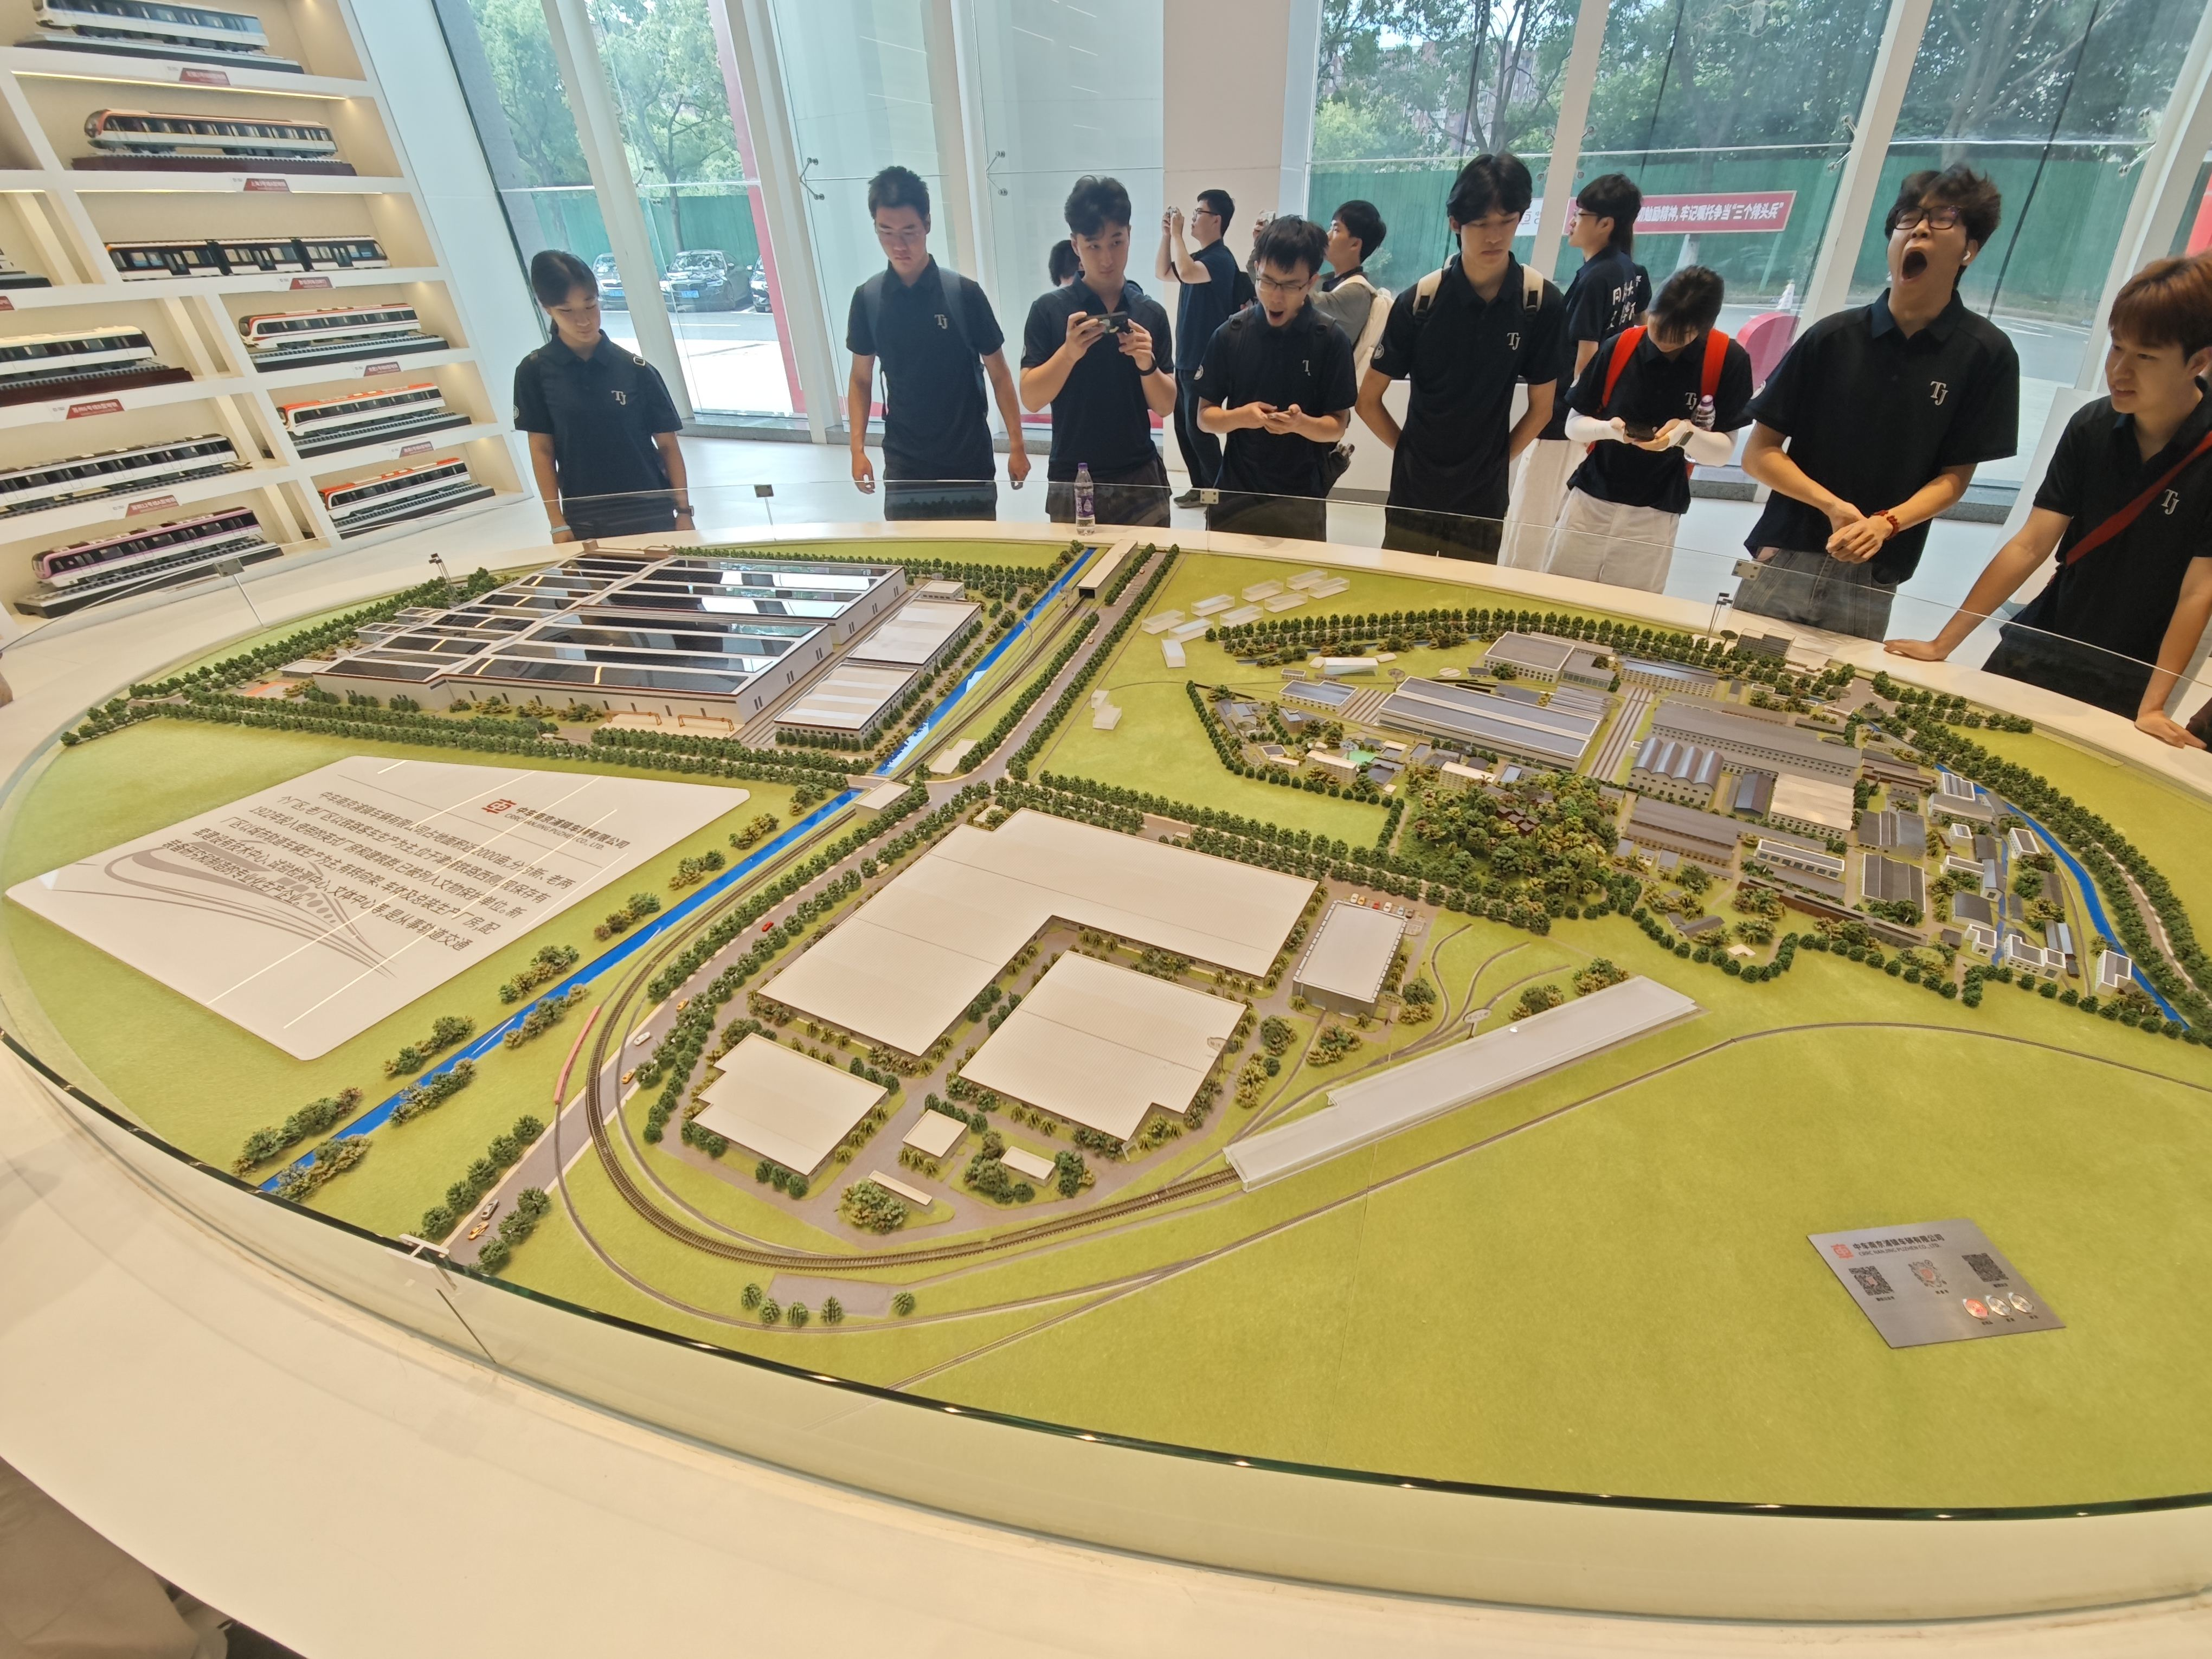
\includegraphics[width=0.8\textwidth]{assets/20260709_122254.jpg}
  \vspace{-0.25cm}
  \caption*{\small{}图1\quad{}厂区模型}
  \vspace{0.25cm}
  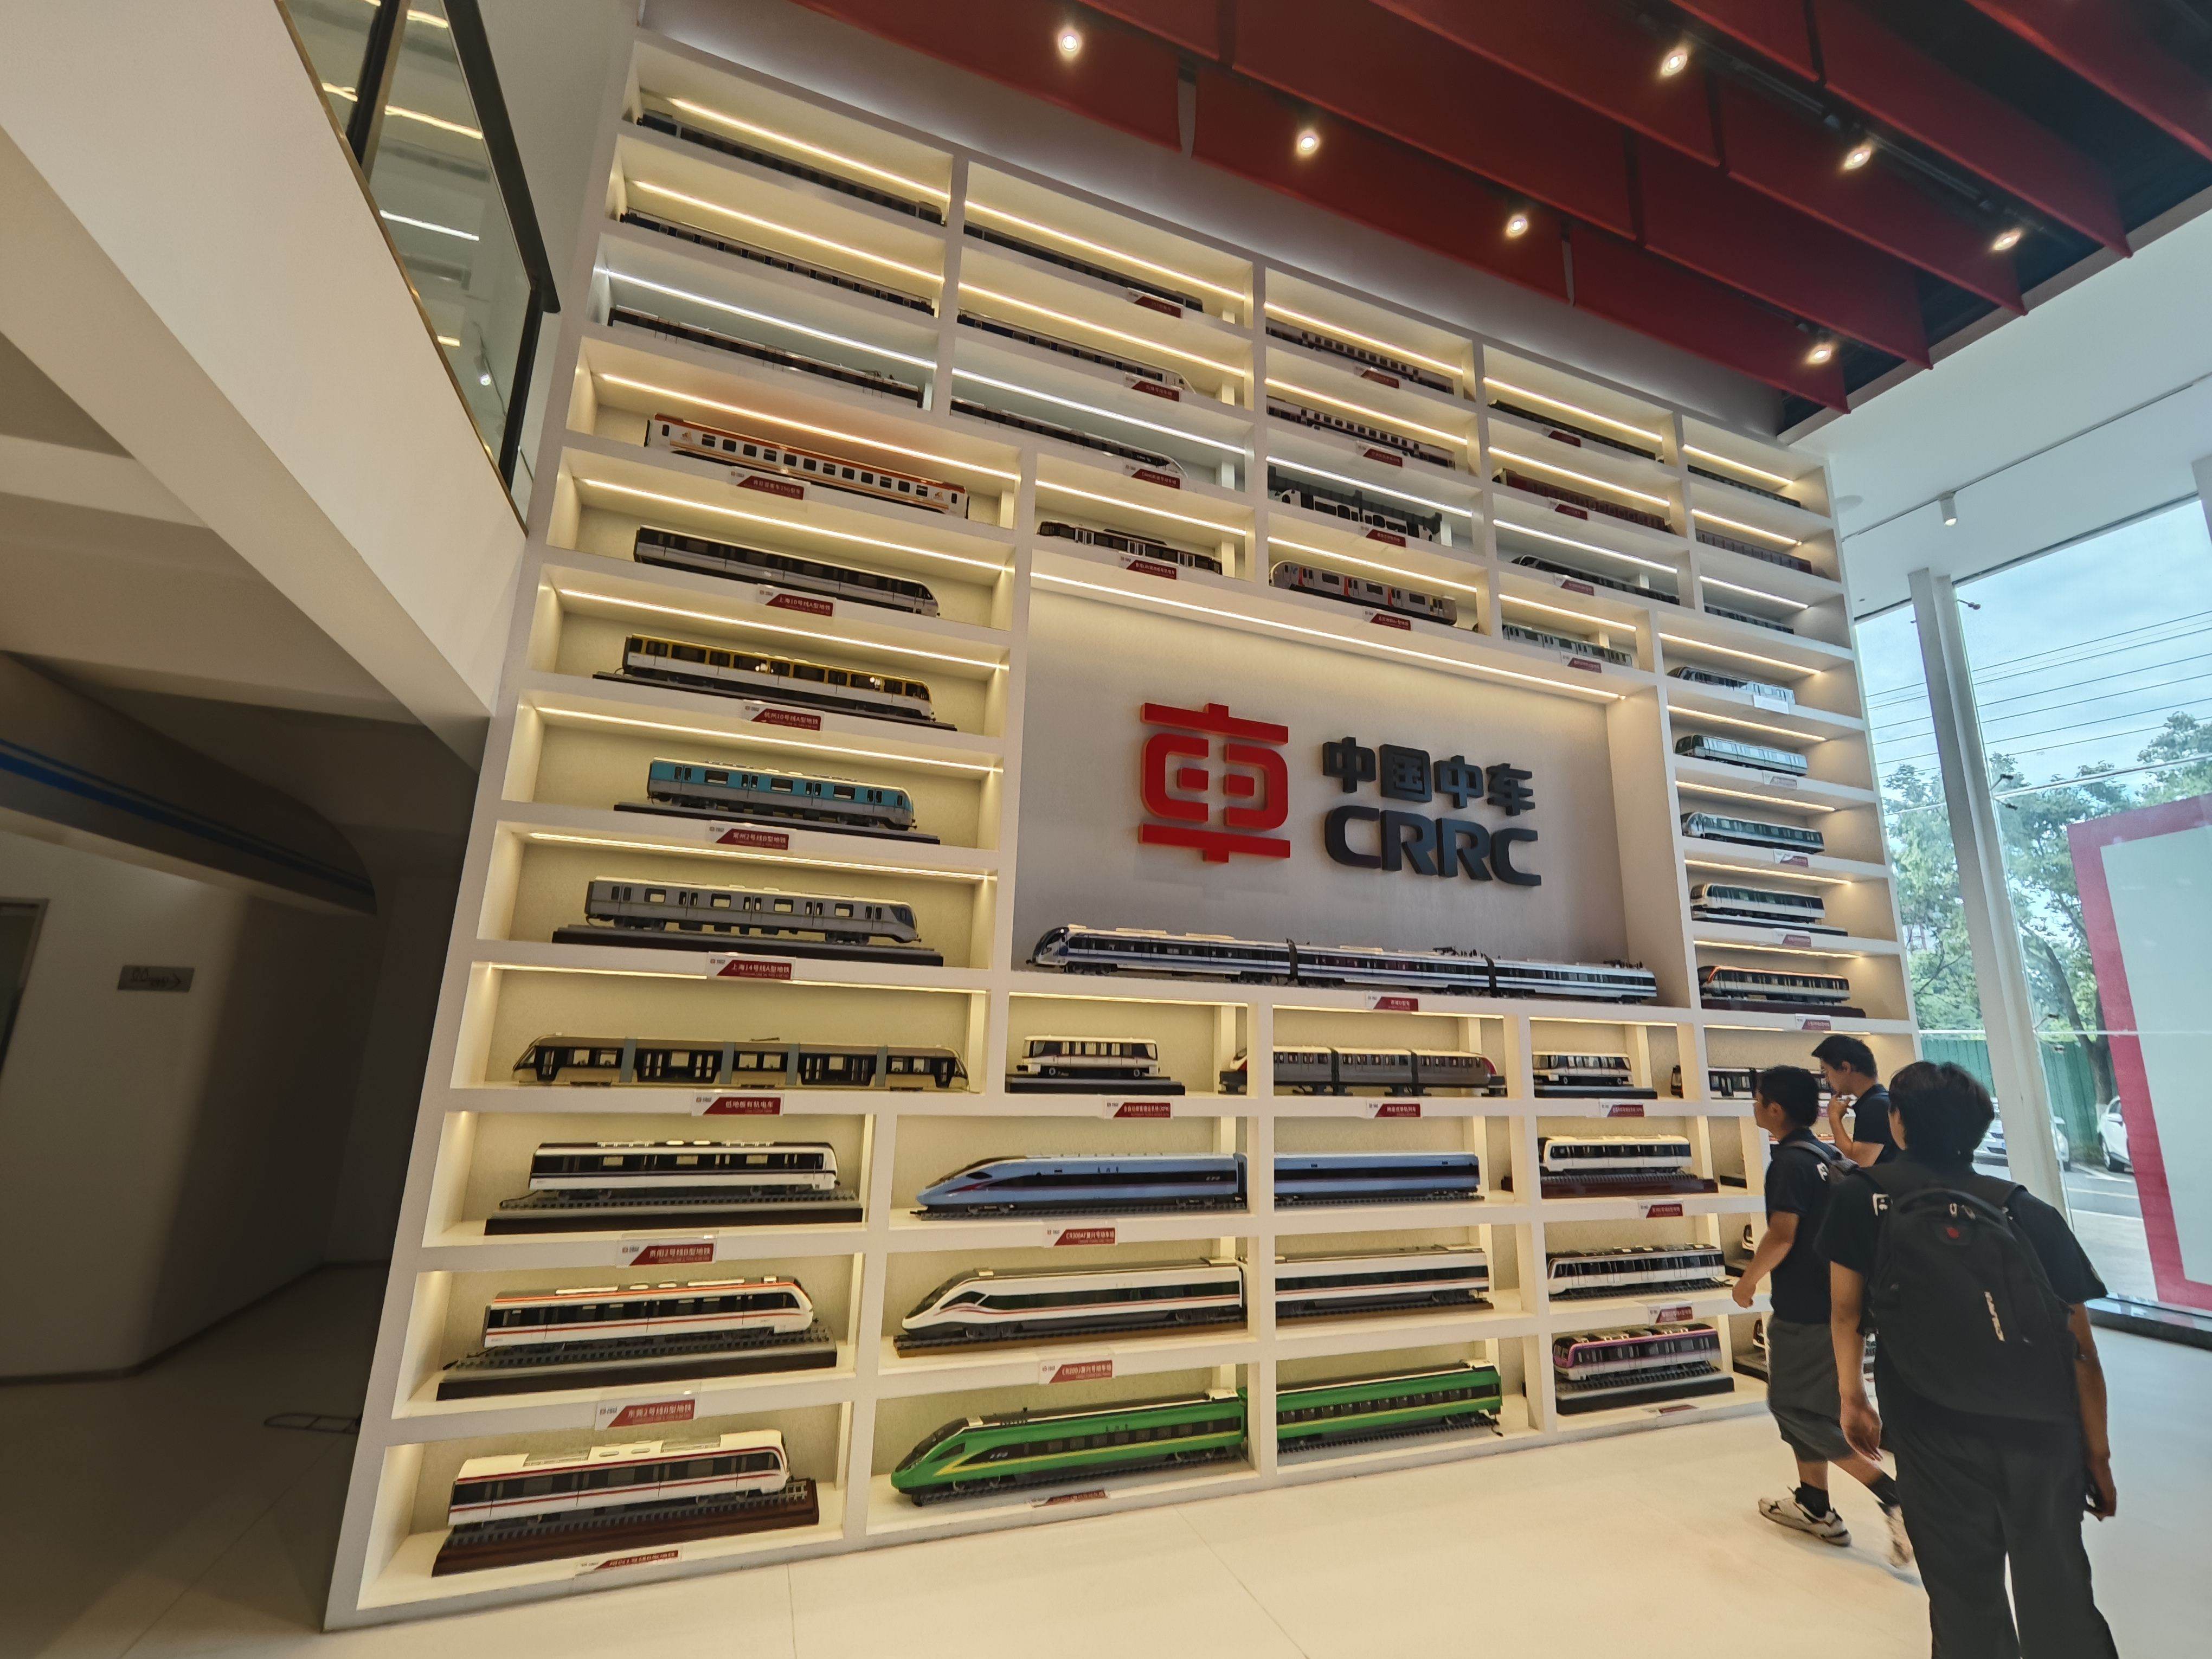
\includegraphics[width=0.8\textwidth]{assets/20260709_122305.jpg}
  \vspace{-0.25cm}
  \caption*{\small{}图2\quad{}浦镇产各式车辆模型}
\end{figure}

\newpage
\journalpage\par\noindent
\begin{figure}[H]
  \centering
  \vspace{2cm}
  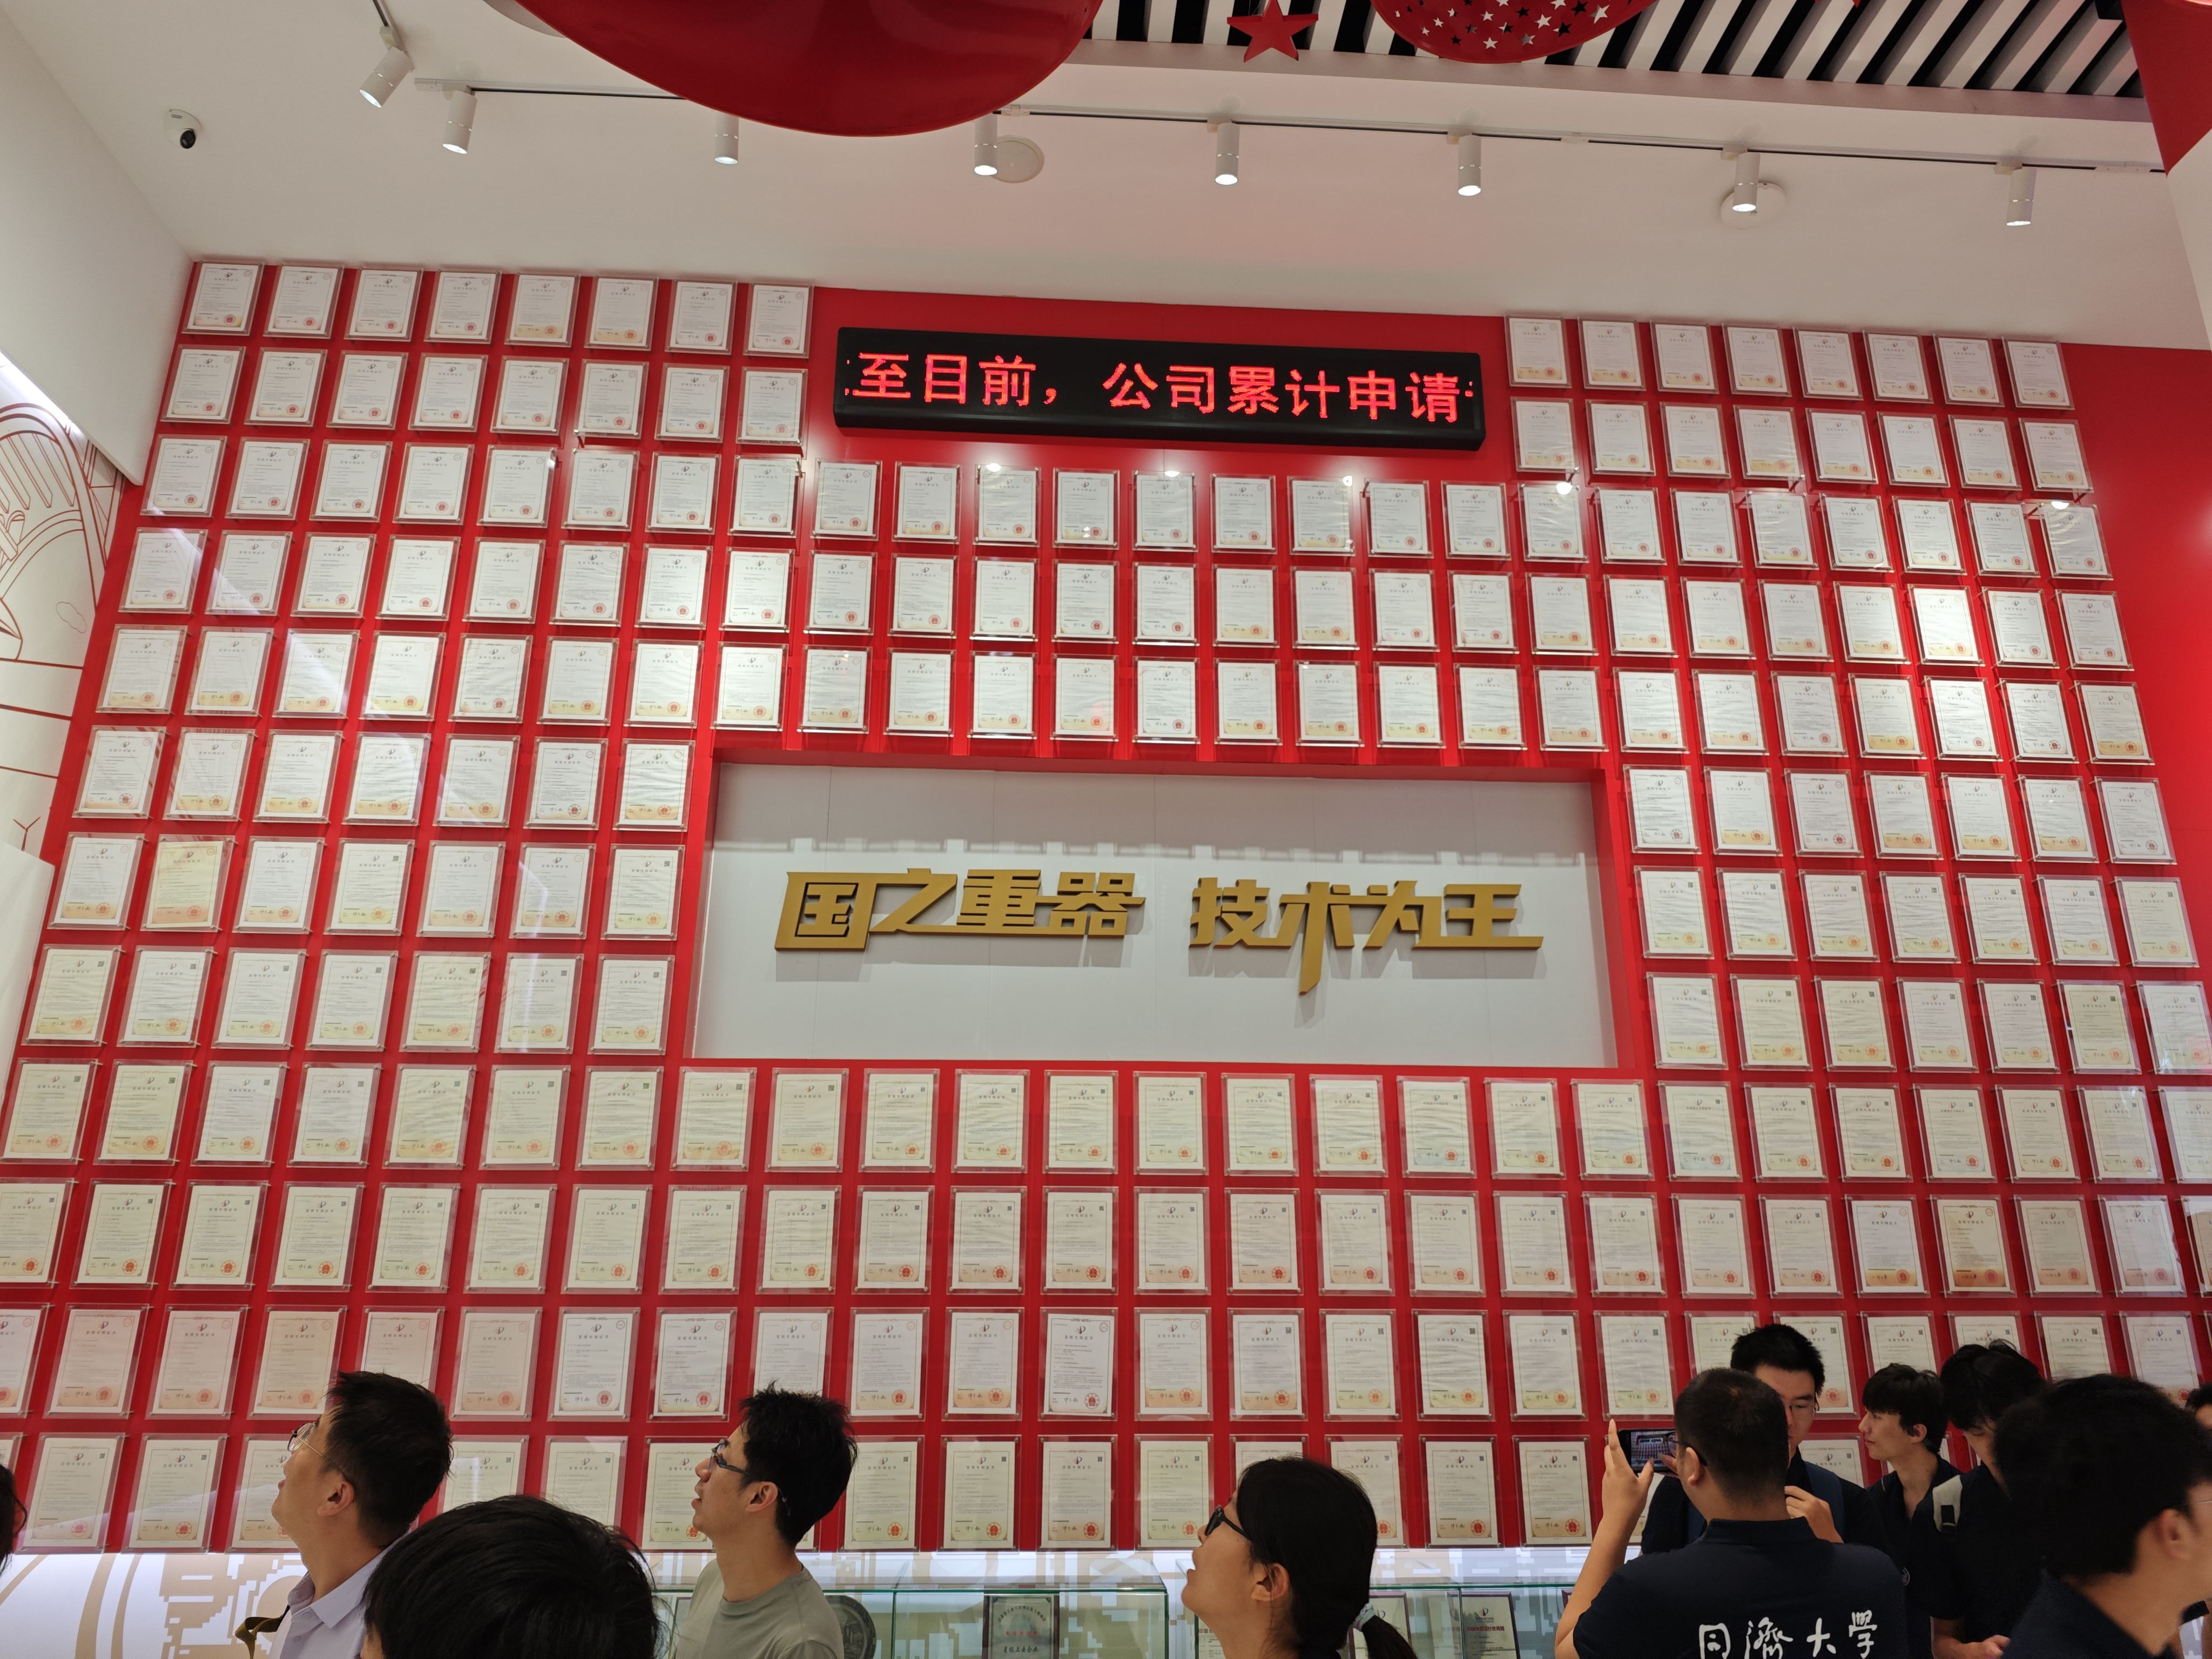
\includegraphics[width=0.8\textwidth]{assets/20260709_122307.jpg}
  \vspace{-0.25cm}
  \caption*{\small{}图3\quad{}浦镇厂获得的各类专利证书}
  \vspace{0.25cm}
  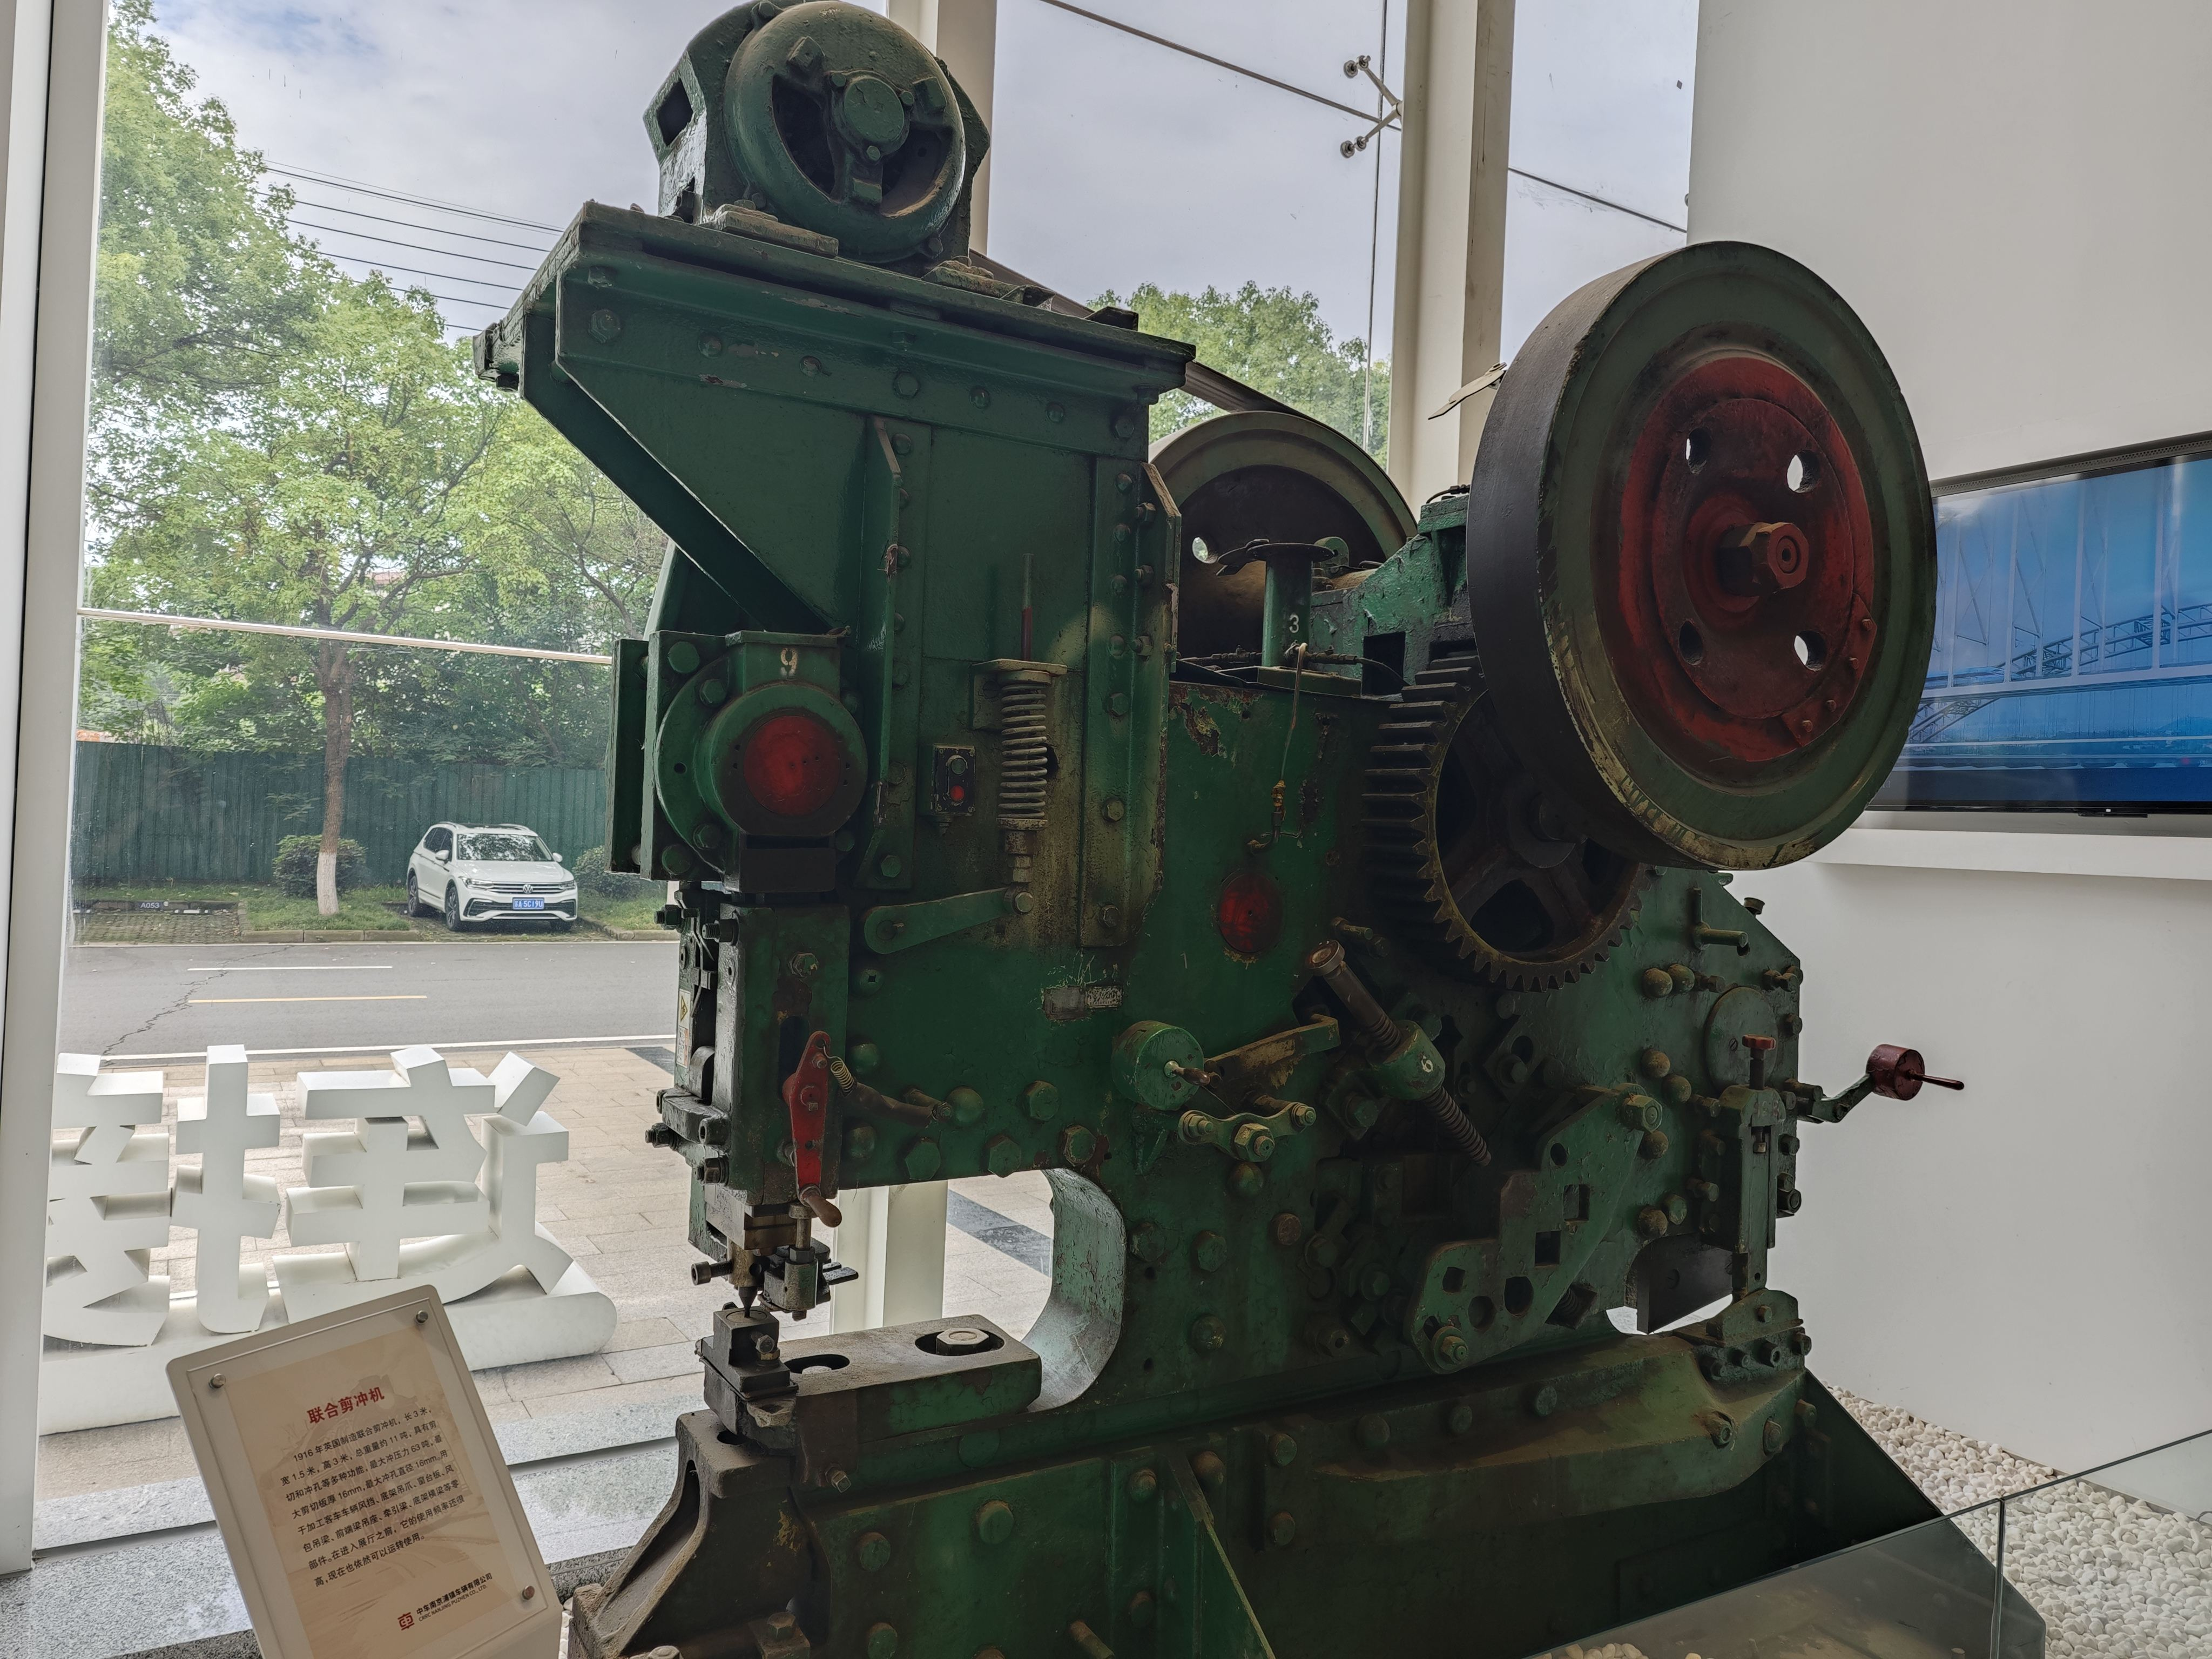
\includegraphics[width=0.8\textwidth]{assets/20260709_122308.jpg}
  \vspace{-0.25cm}
  \caption*{\small{}图4\quad{}浦镇厂老式联合剪冲机（1916年造）}
\end{figure}

\newpage
\journalpage\par\noindent
\begin{figure}[H]
  \centering
  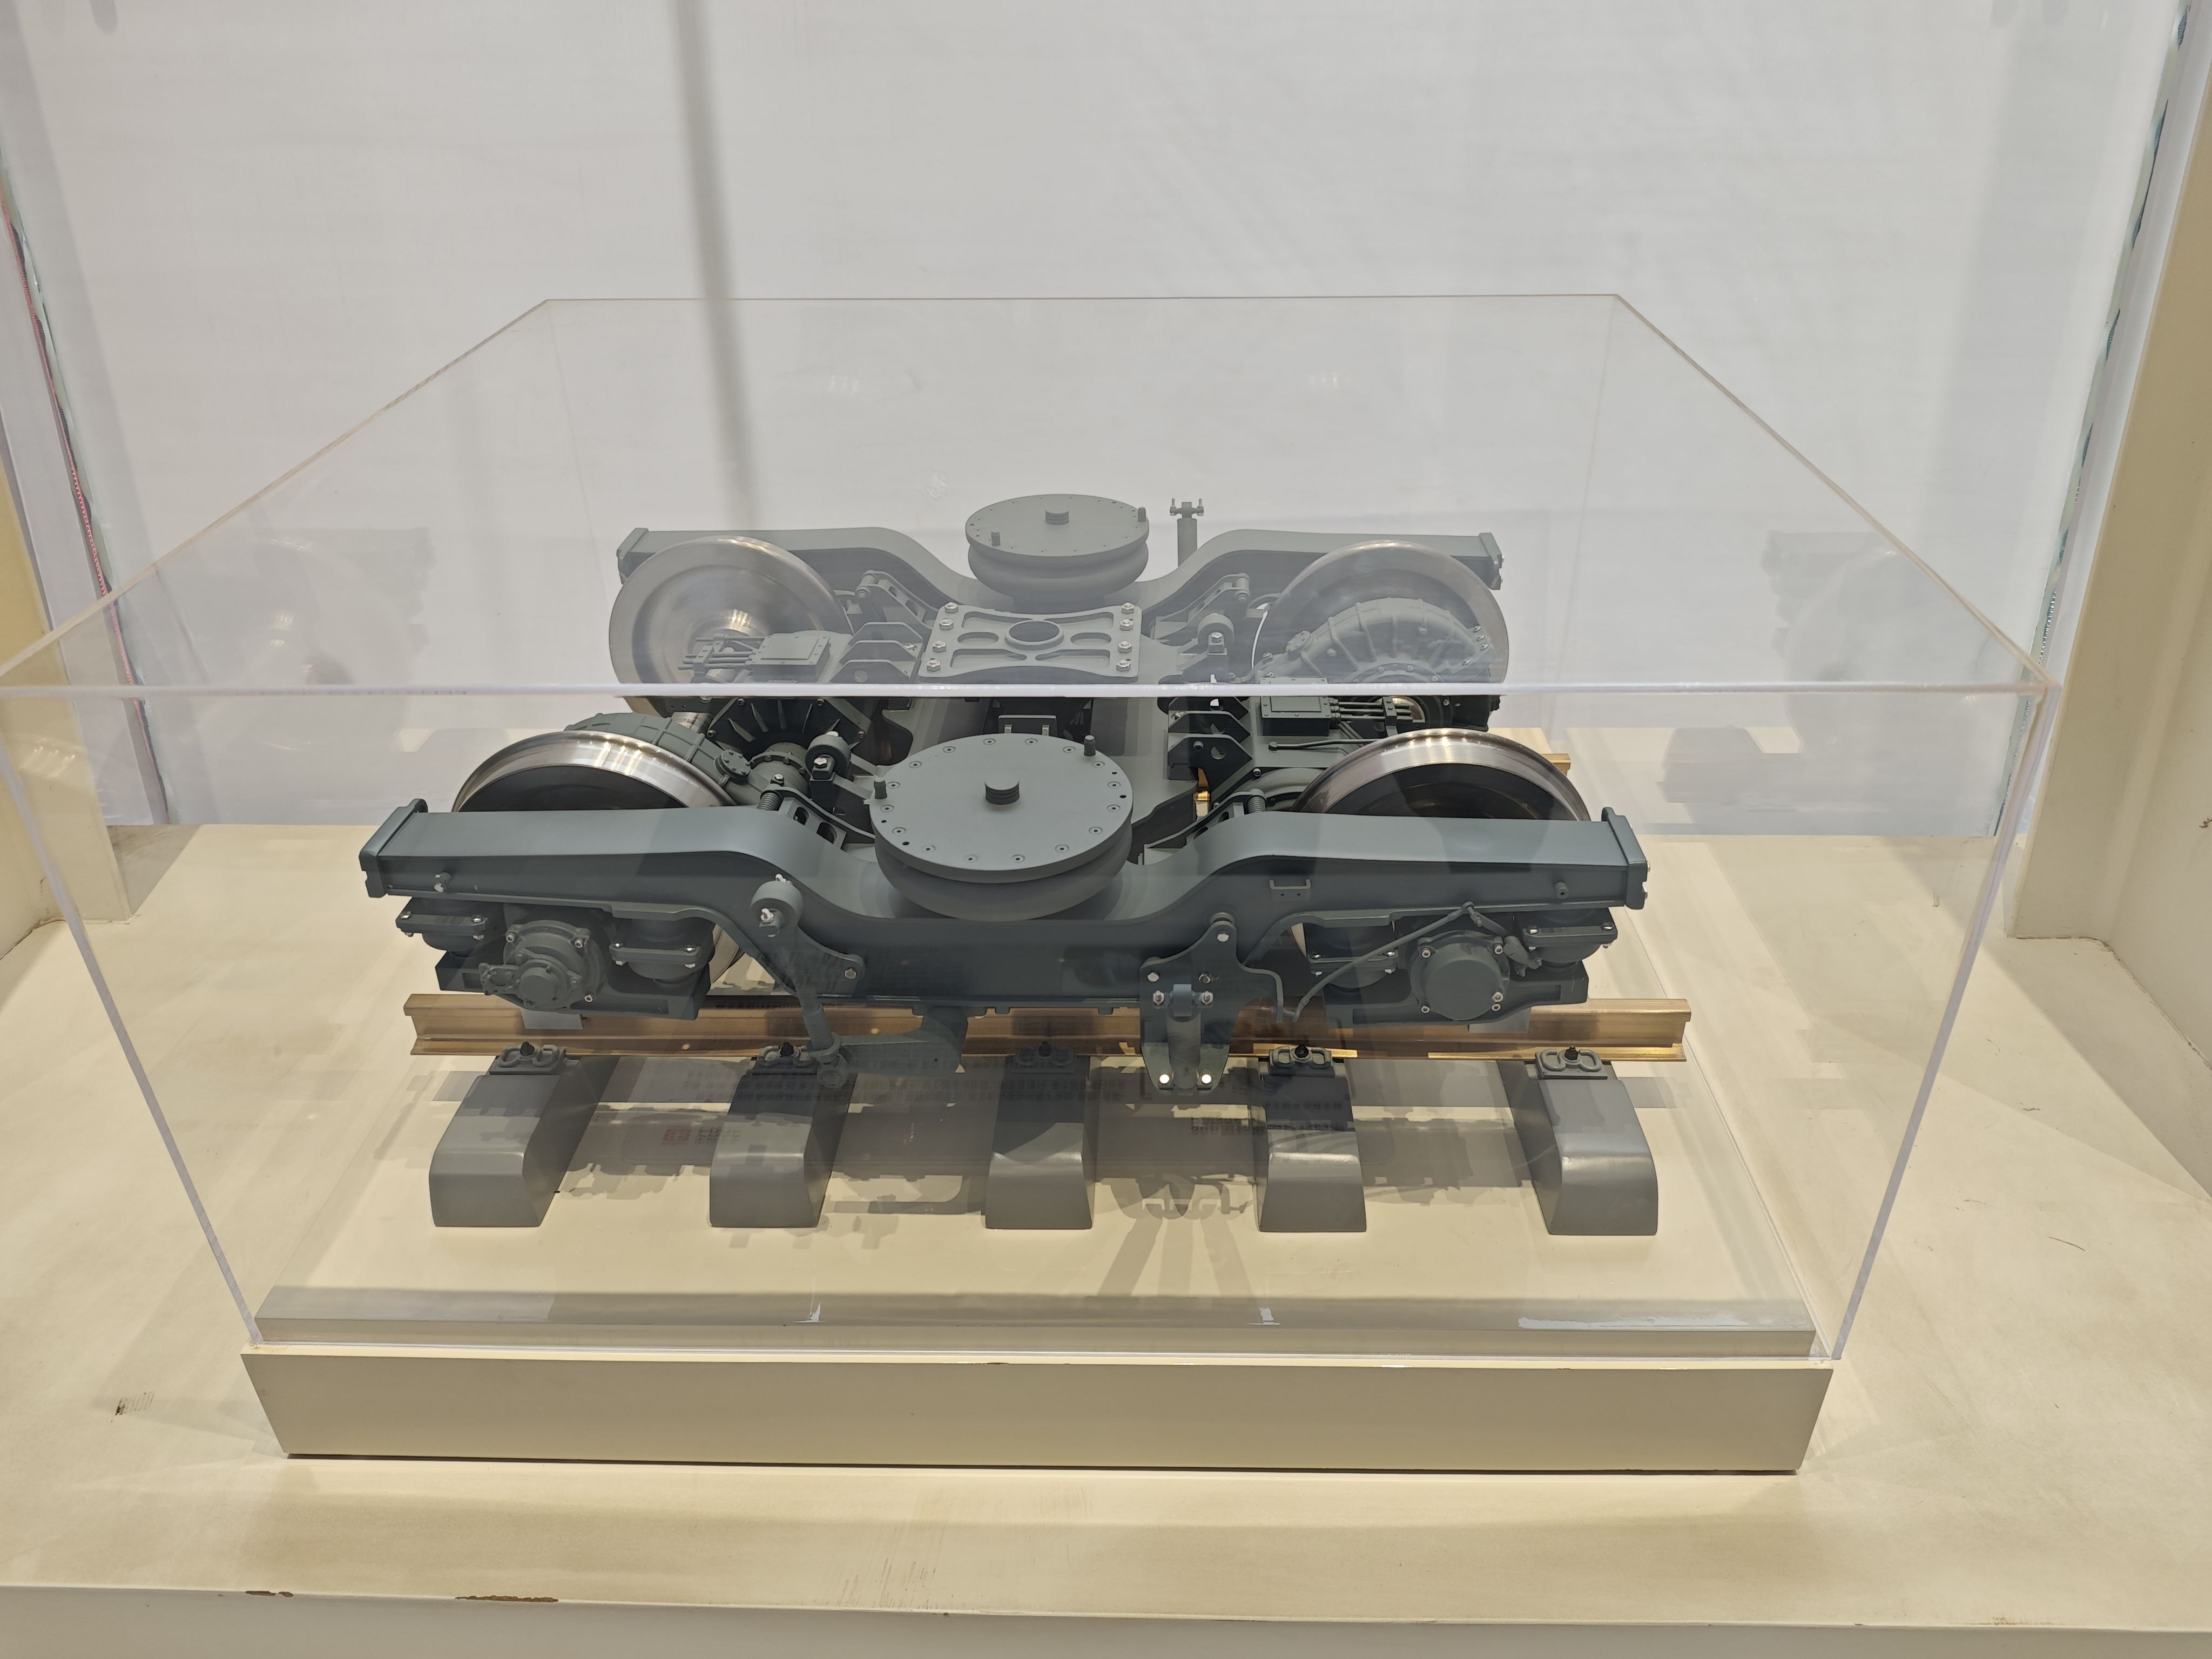
\includegraphics[width=0.8\textwidth]{assets/20260709_122310_2.jpg}
  \vspace{-0.25cm}
  \caption*{\small{}图5\quad{}浦镇产80B型标准地铁转向架PW80E-II}
\end{figure}
\vspace{-0.75cm}\subsection*{二、 转向架分厂参观}\vspace{-0.2cm}
今天剩下的时间我们去了转向架分厂，了解了转向架组装的工艺。\par{}
\vspace{-0.5cm}\subsubsection*{2.1\quad{}转向架整体组装}\vspace{-0.2cm}
转向架组装产线主要有4个工位，分别是节点加装与检测、挂件、落轮和静载/制动性能校验，呈U形排列，如图6：\par{}
\begin{figure}[H]
  \centering
  \vspace{-0.6cm}
  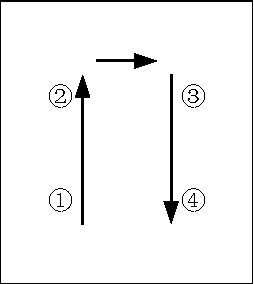
\includegraphics[width=0.25\textwidth, trim=2pt 2pt 2pt 2pt, clip]{assets/U.pdf}
  \vspace{-0.8cm}
  \caption*{\small{}图6\quad{}U形生产线示意图}
  \vspace{-0.5cm}
\end{figure}
第一步顾名思义就是在构架上加装挂设备的节点并进行检测；第二步就是指在转向架构架上加装对应部件，如制动缸的闸线，有正位反位两种放置方法，正位对应正常运行时转向架的上下方向，反位则是倒过来，分别用于安装构架上下两边的部件；第三步是指将转向架安装并紧固到轮对上，浦镇厂中的地铁列车一般采用导柱式和转臂式定位；第四步则是做各种力学性能测试。\par{}
厂内运用了很多智能设备，如前一天提到的智能扳手，可以记录员工与对应工作所使用的扭力等相关信息（一个18万）；员工可通过类似手机的手持终端接收任务或上报情况；检查工作时主要采用自检+互检+专检的“三检”模式，转\par{}

\newpage
\journalpage\par\noindent
向架生产线上共有一百多个停止点，当然也有AI检测，但只作最终确认。\par{}
这里AI辅助检测采用了转向架AI机器视觉外观检测技术，采用非接触式、智能化机器视觉技术，通过图片对比找差，识别标记、防锈油是否异常，是否有异物存在，螺栓有无遮挡等，构建多维度精准感知与决策的“AI大脑”。其搭载六自由度机械臂与地沟多向采集模组，实现检测死角全覆盖；采用3D视觉相机，同步触发采集多维度空间图像数据；植入深度学习算法，对海量图片进行网络训练生成预测模型，实时输出精确检测结论。该设备效益十分明显，直接实现了无人化检测（原需要两人），效率提升了50\%（60 min → 30 min），检出率提升了14\%（85\% → 99\%），并可以自动生成数字化报告，取代了手写纸质报告。\textcolor{gray}{{\bf{}tips: }告示牌原话}\par{}
当然为了保障国企就业岗位，现阶段是绝对不会大量采用机器替代人工的，仅在部分区域少量应用自动化设备。\par{}
\vspace{-0.5cm}\subsubsection*{2.2\quad{}轮对制造}\vspace{-0.2cm}
接着我们又参观了轮对制造产线。轮对是转向架的一个重要组成部分，由轴与轮固结成一个整体，因此轮对制造主要也分为轴和轮两部分。\par{}
首先是轴的制造，先通过车床对毛坯进行粗加工，再通过磨床对轴进行精加工与修正，接着再在一个房间里做探伤检测。\par{}
接着是轮的制造，先对轮饼原料进行加工，再成形打磨其铁屑毛刺等，接着进入预组阶段，即在轮饼与轴接触的内圆上涂抹$\rm MoS_2$润滑脂方便组装。\par{}
再接着就是正式的压装了，由于轴和轮的接触面呈现一个较为细微的锥度（靠近中轴线的部分宽，反之较窄），因此可以直接压紧轮与轴。压装好之后还需要进行测量，如测量轮位差等，防止运行时出现跳动等影响舒适性与耐用性的线性。此外还需要进行装盘（轮盘/轴盘式盘形制动）、清洗、装降噪环等步骤，同时对轴和轮分别进行油漆，并在可能松动旋转的位置布置标记。\par{}
厂里摆放着出口到印度班加罗尔的转向架的轮对，由于当地气候原因，甲方要求在轮饼上和轴上都涂油漆；而国内很少在轮饼上涂，一般都只涂在轴上。\par{}
在组装完轮对之后还要进行轴承的压装、轴箱安装等，有单独的车间进行作业。由于该工序对于温度较为敏感，因此为了防止热胀冷缩导致无法安装，要把轮对与轴承存放至该密闭车间在同一温度下保温8 h，因此该车间是恒温的。\par{}
\vspace{-0.5cm}\subsection*{小结}\vspace{-0.2cm}
今天还是非常充实的一天，学习到了很多知识。厂里到处都是忙碌的生产线和移动的设备、产品，某些讲解的时候恰好遇上作业进行，十分有现场感。可惜由于保密性质，厂房内无法拍照，否则这次的日记会更加丰富。\par{}

\newpage
\journalpage
\vspace{-0.75cm}
\section*{7月8日\quad{}星期三}
\diaryJournalBodyFont\vspace{-0.3cm}\par{}

\newpage
\journalpage
\vspace{-0.75cm}
\section*{7月9日\quad{}星期四}
\diaryJournalBodyFont\vspace{-0.3cm}\par{}

\newpage
\journalpage
\vspace{-0.75cm}
\section*{7月10日\quad{}星期五}
\diaryJournalBodyFont\vspace{-0.3cm}\par{}

\end{document}
